\documentclass[11pt]{article}

\usepackage{../linear}

\begin{document}

\coverpage{5}

% hw problem 1 -----------------------------------------------------------------

\begin{exercise}{1}
    \problem{
        Recall the Power Method algorithm is defined by:
        $$ \boldy _n = A \boldx _n $$
        $$ \lambda _n = \phi (\boldy _n) / \phi (\boldx _n) $$
        $$ \boldx _{n+1} = \boldy _n / \| \boldy _n \| _2 $$
        where $\phi (\boldz) = z_1 + z_2 + \triplecdot + z_n$ and $\boldz = (z_1, z_2, ..., z_n )$.
        For most (but not all) initial guesses $x_0$, $\lambda _n$ will approach the dominant eigenvalue $\lambda$ of $A$ with $x_n$ being an approximation of the associated (unit) eigenvector.
        \begin{enumerate}[label=\alph*)]
            \item Let
            $$ A = \begin{bmatrix} 7 & 3 \\ 3 & -1 \end{bmatrix}
            \hspace{3em}
            \boldx_0 = \begin{pmatrix} 1 \\ -3 \end{pmatrix} $$
            Using hand calculations (no decimal approximations) only, compute in sequence $\boldy _0, \lambda _0, \boldx _1, \boldy _1, \lambda _1, \boldx _2$.
            You should find $\boldx _1 = - \boldx _2$.
            Is the method converging to the dominat eigenvalue?
            Give some reasonable explanation.
            \item Let
            $$ A =
            \begin{bmatrix}
                16 & 2 & 4 \\
                1 & 40 & -3 \\
                0 & 3 & 5
            \end{bmatrix}
            \hspace{3em}
            \boldx _0 =
            \begin{pmatrix} 1 \\ 1 \\ 1 \end{pmatrix}
            $$
            Use the posted \textit{Power.m} and \textit{phi.m} matlab scripts to approximate the dominant eigenvalue using $N = 15$ iterates.
            Include an extra column in the output matrix $R$ as follows.
            $$ >> R = [ x', lambda(k), residual(k), abs(r-edom) ] $$
            where $edom$ is the dominant eigenvalue.
            You may find this value using the matlab statement
            $$ >> evals = eig(A) $$
            where $evals$ is a vector of all the eigenvalues of $A$.
        \end{enumerate}
        \hspace{0em}
    }
    \answer{
        \begin{enumerate}[label=\alph*)]
            \item Now we show the computations for $y_0, \lambda _0, x_1, y_1, \lambda _1, x_2$:
            $$ y_0 = A x_0 = \begin{bmatrix} 7 & 3 \\ 3 & -1 \end{bmatrix} \begin{pmatrix} 1 \\ -3 \end{pmatrix} = \begin{pmatrix} 7-9 \\ 3+3 \end{pmatrix} = \begin{pmatrix} -2 \\ 6 \end{pmatrix} $$
            $$ \lambda _0 = \phi(y_0) / \phi(x_0) = \dfrac{-2+6}{1+-3} = \dfrac{4}{-2} = -2 $$
            $$ x_1 = \dfrac{y_0}{\| y_0 \| _2} = \dfrac{1}{\sqrt{2^2 + 6^2}} \begin{pmatrix} -2 \\ 6 \end{pmatrix} = \dfrac{1}{2\sqrt{10}} \begin{pmatrix} -2 \\ 6 \end{pmatrix} = \begin{pmatrix} -1/\sqrt{10} \\ 3/\sqrt{10} \end{pmatrix} $$
            $$ y_1 = A x_1 = \begin{bmatrix} 7 & 3 \\ 3 & -1 \end{bmatrix} \begin{pmatrix} -1/\sqrt{10} \\ 3 / \sqrt{10} \end{pmatrix} = \begin{pmatrix} -7/\sqrt{10} + 9/\sqrt{10} \\ -3/\sqrt{10} - 3/\sqrt{10} \end{pmatrix} = \begin{pmatrix} 2/\sqrt{10} \\ -6/\sqrt{10} \end{pmatrix} $$
            $$ \lambda _1 = \phi (y_1) / \phi (x_1) = \dfrac{2/\sqrt{10} - 6\sqrt{10}}{-1/\sqrt{10} + 3/\sqrt{10}} = \dfrac{-4/\sqrt{10}}{2/\sqrt{10}} = -2 $$
            $$ x_2 = \dfrac{y_1}{\| y_1 \| _2} = \dfrac{1}{\sqrt{(4/\sqrt{10})^2 + (6/\sqrt{10})^2}} \begin{pmatrix} 2/\sqrt{10} \\ -6/\sqrt{10} \end{pmatrix} = \dfrac{1}{2} \begin{pmatrix} 2/\sqrt{10} \\ -6/\sqrt{10} \end{pmatrix} = \begin{pmatrix} 1/\sqrt{10} \\ -3/\sqrt{10} \end{pmatrix} $$
            Because $\boldx _1 = - \boldx _2 = \begin{pmatrix} -1/\sqrt{10} \\ 3/\sqrt{10} \end{pmatrix} $, we can conclude that our initial guess $\boldx _0$ was an eignvector.
            This means that $\lambda _1 = \lambda _2 = -2$ is an eigenvalue.
            To say whether $-2$ is the dominant eigenvalue, we will compute the eigenvalues of $A$:
            $\det (A - \lambda I) = (7-\lambda)(-1 - \lambda) - 9 = \lambda ^2 - 6 \lambda - 16 = (\lambda - 8)(\lambda + 2) $.
            So the eigenvalues are $8$ and $-2$, therefore $-2$ is not the dominant eigenvalue.
            My reasoning as to why $-2$ is not the dominant eigenvalue for $A$ does not generalize well to higher dimensions since it defeats the whole point of an iterative method (which is supposed to be faster than finding the actual eigenvalues), but it suffices for this example.
            \item Using \textit{Power.m} and \textit{phi.m}, I found an approximation for the dominant eigenvalue as 39.839856538994297.
            Here is the output matrix $R$ from matlab:
            {\scriptsize
            \begin{center}
                \begin{tabular}{|c|c|c|c|c|c|}
                    \hline
                    eigenvector & & & eigenvalue & residual & absolute error \\ \hline
                    1.000000000000000  &  1.000000000000000 &  1.000000000000000 & - &                  -                  &  - \\ \hline
                    0.492921786443043  &  0.851410358401620 &  0.179244285979288 & 22.666666666666668 & 14.751171305567953 &  17.173349870446248 \\ \hline
                    0.288650126609190  & 0.952545417810325  & 0.096635042386555 & 31.352941176470587  & 8.514642897746276  & 8.487075360642329 \\ \hline
                    0.177791416892457  & 0.980306869857993  & 0.085957274204090 & 36.141651031894931  & 3.925083655344991  & 3.698365505217986 \\ \hline
                    0.129984672450642  & 0.987858078096879  & 0.085090554508944 & 38.303760998780064  & 1.661447031042967  & 1.536255538332853 \\ \hline
                    0.110508604618063  & 0.990216709359014  & 0.085198103333200 & 39.215720501528395  & 0.679404750869178  & 0.624296035584521 \\ \hline
                    0.102696155271591  & 0.991048657684767  & 0.085299811216993 & 39.589054515969927  & 0.273690124388765  & 0.250962021142989 \\ \hline
                    0.099577137816148  & 0.991362763435785  & 0.085347905055174 & 39.739652038687048  & 0.109532584310219  & 0.100364498425868 \\ \hline
                    0.098333871704795  & 0.991485123035684  & 0.085368029580514 & 39.799973167105179  & 0.043712123870553  & 0.040043370007737 \\ \hline
                    0.097838568980598  & 0.991533420743819  & 0.085376167446719 & 39.824056566750471  & 0.017423731934735  & 0.015959970362445 \\ \hline
                    0.097641285388108  & 0.991552587293665  & 0.085379423861936 & 39.833658239997888  & 0.006941658824055  & 0.006358297115028 \\ \hline
                    0.097562711262609  & 0.991560209754089  & 0.085380722669200 & 39.837483927715994  & 0.002765001745509  & 0.002532609396923 \\ \hline
                    0.097531417599642  & 0.991563243776705  & 0.085381240164471 & 39.839007837873581  & 0.001101261844997  & 0.001008699239335 \\ \hline
                    0.097518954420133  & 0.991564451842739  & 0.085381446290237 & 39.839614800735262  & 0.000438602067464  & 0.000401736377654 \\ \hline
                    0.097513990787375  & 0.991564932927385  & 0.085381528385413 & 39.839856538994297  & 0.000174680576074  & 0.000159998118619 \\ \hline
                \end{tabular}
            \end{center}
            }
            Here is a larger version of the above table with only the eigenvalue approximation and the absolute error.
            \begin{center}
                \begin{tabular}{|c|c|c|c|c|c|}
                    \hline
                    eigenvalue & absolute error \\ \hline
                    - &                  - \\ \hline
                    22.666666666666668  &  17.173349870446248 \\ \hline
                    31.352941176470587  & 8.487075360642329 \\ \hline
                    36.141651031894931  & 3.698365505217986 \\ \hline
                    38.303760998780064  & 1.536255538332853 \\ \hline
                    39.215720501528395  & 0.624296035584521 \\ \hline
                    39.589054515969927  & 0.250962021142989 \\ \hline
                    39.739652038687048  & 0.100364498425868 \\ \hline
                    39.799973167105179  & 0.040043370007737 \\ \hline
                    39.824056566750471  & 0.015959970362445 \\ \hline
                    39.833658239997888  & 0.006358297115028 \\ \hline
                    39.837483927715994  & 0.002532609396923 \\ \hline
                    39.839007837873581  & 0.001008699239335 \\ \hline
                    39.839614800735262  & 0.000401736377654 \\ \hline
                    39.839856538994297  & 0.000159998118619 \\ \hline
                \end{tabular}
            \end{center}
        \end{enumerate}
    }
\end{exercise}

Here is the matlab code used to generate the above tables.
\begin{Verbatim}
%%%%%%%%%%%%%%%%%%%%%%%%%%%%%%%%%%%%%%%%%%%%%%%%
%
%  Power Method : Define problem here
%
%       A = matrix
%      x0 = initial (dominant) eigenvector guess
%           define as a column vector.
%
%             r = current estimate of dominant eigenvalue
%             x = current estimate of unit eigenvector
%             N = number of iterates
%     lambda(k) = k-th approximate value of dom. e-val
%  residual(k)  = 2-norm of Ax-rx at k-th iterate
%        R(k,:) = k-th approximate e-vector, lambda(k),
%                 residual(k),absolute error of for dom. eval
%
%
format long

A=[16,2,4;1,40,-3;0,3,5];
x0=[1;1;1];
evals=eig(A);
edom=evals(1);

N=15;
R(1,:)=[x0',0,0,0];

x=x0;
for k=2:N
  y=A*x;
  r=phi(y)/phi(x);
  x=y/norm(y);
  lambda(k)=r;
  residual(k)=norm(A*x-r*x,2);
  R(k,:)=[x',lambda(k),residual(k),abs(r-edom)];
end;
%
disp('  ')
disp('  ')
disp('   eigenvector - lambda - residual - absolute error')
disp('  ')
R
\end{Verbatim}

\newpage

\newcommand{\matA}{\begin{bmatrix} 2 & 1/4 \\ 1/4 & 1/2 \end{bmatrix}}
\newcommand{\vectorb}{\begin{pmatrix} 1 \\ 2 \end{pmatrix}}
\newcommand{\xnaught}{\begin{pmatrix} 0 \\ 0 \end{pmatrix}}
\newcommand{\rnaught}{\begin{pmatrix} -1 \\ -2 \end{pmatrix}}
\newcommand{\rnaughtT}{\begin{pmatrix} -1 & - 2 \end{pmatrix}}
\newcommand{\xone}{\begin{pmatrix} 1 \\ 2 \end{pmatrix}}
\newcommand{\rone}{\begin{pmatrix} 3/2 \\ -3/4 \end{pmatrix}}
\newcommand{\roneT}{\begin{pmatrix} 3/2 & -3/4 \end{pmatrix}}
\newcommand{\xtwo}{\begin{pmatrix} 0 \\ 5/2 \end{pmatrix}}

% hw problem 2 -----------------------------------------------------------------

\begin{exercise}{2}
    \problem{
        Recall that the steepest descent algorithm for approximating the solution of $Ax = b$ (when $A = A^T$ is positive definite) is
        $$\boldr _n = A\boldx _n - \boldb$$
        $$\alpha _n = \dfrac{\boldr ^T_n \boldr _n}{\boldr ^T_n A \boldr _n} $$
        $$\boldx _{n+1} = \boldx _n - \alpha _n \boldr _n $$
        where $\boldr _n$ is the residual vector and $\boldx _n$ is the approximation of the solution $Ax = b$.
        \begin{enumerate}[label=\alph*)]
            \item Let
            $$ A = \begin{bmatrix} 2 & 1/4 \\ 1/4 & 1/2 \end{bmatrix}
            \hspace{2em}
            \boldb = \begin{pmatrix} 1 \\ 2 \end{pmatrix}
            \hspace{2em}
            \boldx _0 = \begin{pmatrix} 0 \\ 0 \end{pmatrix} $$
            First prove $A$ is positive definite and then use hand calculations (no decimal approximations) to compute in sequence $\boldr _0, \alpha _0, \boldx_1, \boldr _1, \alpha _1, \boldx _2$.
            \item Use the code $steepest.m$ to approximate the solution of $Ax = b$ where $A \in \R ^{50 \times 50}$ is the tri-diagonal matrix defined on the assignment sheet.
            The iterat output in $steepest.m$ is stored in the matrix $R$.
            $$ R(n,:) = [n, xn', norm(en,2)];$$
            The last comlumn of $R$ is the 2-norm of the absolute error.
            Plot this absolute error versus iteration number for $N = 3000$ iterates.
            Use matlab to do this.
        \end{enumerate}
        \hspace{0em}
    }
    \answer{
        \begin{enumerate}[label=\alph*)]
            \item Now we show the computations for $\boldr_0, \alpha _0, \boldx_1, \boldr_1, \alpha _1, \boldx_2$:
            $$ \boldr_0 = A \boldx_0 - \boldb = \matA \xnaught - \vectorb = \xnaught - \vectorb = \begin{pmatrix} -1 \\ -2 \end{pmatrix} $$
            $$ \alpha _0 = \dfrac{\boldr_0^T \boldr_0}{\boldr_0^T A \boldr_0} = \dfrac{\rnaughtT \rnaught}{\rnaughtT \matA \rnaught} = \dfrac{1 + 4}{\rnaughtT \begin{pmatrix} -5/2 \\ -5/4 \end{pmatrix}} = \dfrac{5}{5/2 + 5/2} = 5/5 = 1 $$
            $$ \boldx_1 = \boldx_0 - \alpha _0 \boldr_0 = \xnaught - 1 \rnaught = \vectorb $$
            $$ \boldr_1 = A \boldx_1 - \boldb = \matA \xone - \vectorb = \begin{pmatrix} 5/2 \\ 5/4 \end{pmatrix} - \vectorb = \rone $$
            $$ \alpha _1 = \dfrac{\boldr_1^T \boldr_1}{\boldr_1^T A \boldr_1} = \dfrac{\roneT \rone}{\roneT \matA \rone} = \dfrac{9/4 + 9/16}{\roneT \begin{pmatrix} 45/16 \\ 0 \end{pmatrix}} = \dfrac{45/16}{3/2 * 45/16} = 2/3 $$
            $$ \boldx_2 = \boldx_1 - \alpha _1 \boldr_1 = \xone - 2/3 \rone = \xone - \begin{pmatrix} 1 \\ -1/2 \end{pmatrix} = \xtwo $$ \newpage
            \item Using \textit{steepest.m}, I found an approximation an approximation for $x$ in $Ax = b$ where $A$ is the $50 \times 50$ tridiagonal matrix defined on the assignment sheet.
            Here is the plot matlab generated for error vs the number of iterates.
            The code that I used is on the next page.
            \begin{figure}[h]
                \begin{center}
                    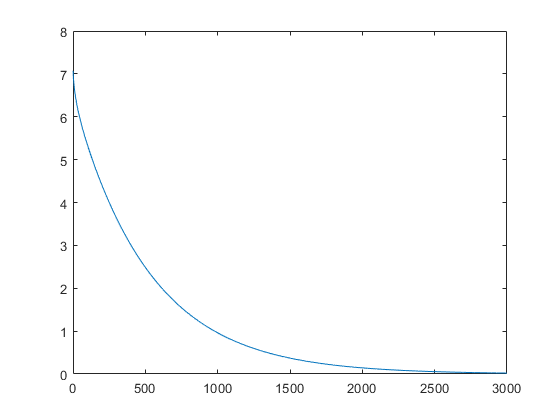
\includegraphics[scale=1]{plot}
                    \caption{Error vs Number of iterates}
                    \label{fig:plot}
                \end{center}
            \end{figure}
        \end{enumerate}
    }
\end{exercise}

\newpage
\begin{Verbatim}
    % Steepest descent method:
    %            Ax = b
    clear all;
    format long
    M=50;
    a=2;
    am=-1;
    ap=-1;
    A=diag(a*ones(1,M))+diag(ap*ones(1,M-1),1)+diag(am*ones(1,M-1),-1);
    xbar=ones(M,1); % exact solution
    b=A*xbar;
    xn=zeros(M,1); % initial guess
    N=3000;
    for n=1:N
        rn=A*xn-b;
        an=(rn'*rn)./(rn'*(A*rn));
        xnp=xn-an*rn;
        en=xn-xbar;
        R(n,:)=[n,xn',norm(en,2)];
        xn=xnp;
    end
    len=length(R(1,:));
    plot(R(:,len));
\end{Verbatim}

\end{document}
